 % mainfile: ../../../../master.tex
\subsection{Migrate Zicheng's code}
\label{task:20240305_aosp}

\subsubsection{Code differencing}

\begin{longtable}{p{.15\linewidth}p{.40\linewidth}p{.40\linewidth}} 
\toprule
file & 13 to Debloated 13 & 13 to 14 \\
\midrule
\endhead

\path{art_dex_file_loader.cc}
& No change
& Removed MemMapContainer. Replace \texttt{DexFileLoader::OpenCommon} now protected with \texttt{ArtDexFileLoader::Open}, and remove its other overloads.
\\

\path{dex_file_loader.cc}
& No change
& Remove \texttt{DexFileLoader::GetMultiDexChecksums}, \texttt{DexFileLoader::OpenAll}, \texttt{DexFileLoader::OpenOneDexFileFromZip}, \texttt{DexFileLoader::OpenAllDexFilesFromZip}. Modified \texttt{DexFileLoader::Open} and added its overloads, \texttt{DexFileLoader::OpenCommon} and added its overloads. Added \texttt{DexFileLoader::InitAndReadMagic}, \texttt{DexFileLoader::OpenWithDataSection}, \texttt{DexFileLoader::OpenFromZipEntry}
\\

\path{native_loader.cpp}
& Trivial loggings
& No change
\\

\path{native_loader_namespace.cpp}
& Trivial loggings
& No change
\\

\path{odrefresh.cc}
& Change from \path{args.emplace_back("--compiler-filter=speed");} to \path{args.emplace_back("--compiler-filter=verify");}
& Tons of change
\\

\path{quick_trampoline_entrypoints.cc}
& No change
& Lots of change
\\

\path{interpreter_common.cc}
& Trivial Logging
& Modified \path{ShouldStayInSwitchInterpreter}, \path{MoveToExceptionHandler}, \path{DoCallCommon}, \path{ArtInterpreterToCompiledCodeBridge}, \path{InvokeBootstrapMethod}, \path{DoCall}. Added \path{UnlockHeldMonitors}
\\

\path{interpreter_switch.cc}
& Trivial JNI headers imported
& Modified \path{ShouldStayInSwitchInterpreter}, \path{MoveToExceptionHandler}, \path{DoCallCommon}, \path{ArtInterpreterToCompiledCodeBridge}, \path{InvokeBootstrapMethod}, \path{DoCall}. Added \path{UnlockHeldMonitors}
\\

\path{interpreter_switch_impl-inl.h}
& Trivial JNI headers imported
& Modified template settings for \path{CheckTransactionAbort}, \path{CheckForceReturn}, \path{HandlePendingException}, \path{HandleReturn}, \path{HandleGet}, \path{HandlePut}, \path{HandleInvoke}, \path{RETURN_OBJECT}, \path{MONITOR_ENTER}, \path{MONITOR_EXIT}, \path{NEW_ARRAY}, \path{FILLED_NEW_ARRAY}, \path{FILLED_NEW_ARRAY_RANGE}, \path{ExecuteSwitchImplCpp}. Modified \path{Preamble}, \path{CONST_CLASS}, \path{CHECK_CAST}, \path{INSTANCE_OF}, \path{NEW_INSTANCE}, \path{THROW}, \path{CHECK_CAST}. Added \path{DoAssignabilityChecks}
\\

\path{interpreter_switch_impl.h}
& Trivial logging headers imported
& Modified template settings for \path{ExecuteSwitchImplCpp}, \path{ExecuteSwitchImpl}.
\\

\path{interpreter.cc}
& No changes
& Modified \path{ExecuteSwitch}, \path{Execute}, \path{EnterInterpreterFromInvoke}, \path{EnterInterpreterFromDeoptimize}, \path{EnterInterpreterFromEntryPoint}.
\\

\path{jit.cc}, \path{jit_code_cache.cc}
& No changes
& Changes
\\

\path{java_vm_ext.cc}
& Modified \path{FindSymbol} to check if MINIMA symbol
& Modified \texttt{JavaVMExt::JavaVMExt},  \texttt{JavaVMExt::Create},  \texttt{JavaVMExt::AddGlobalRef},  \texttt{JavaVMExt::AddWeakGlobalRef}, \texttt{JavaVMExt::DeleteGlobalRef}, \texttt{JavaVMExt::DeleteWeakGlobalRef}, \texttt{JavaVMExt::DisallowNewWeakGlobals}, \texttt{JavaVMExt::AllowNewWeakGlobals}, \texttt{JavaVMExt::DecodeGlobal}, \texttt{JavaVMExt::GetIndirectRefKind}, \texttt{JavaVMExt::DecodeWeakGlobalDuringShutdown}, \texttt{JavaVMExt::LoadNativeLibrary}, \texttt{JavaVMExt::FindCodeForNativeMethod}, \texttt{JavaVMExt::GetLibrarySearchPath}. Added \texttt{JavaVMExt::Initialize}, \texttt{JavaVMExt::DecodeWeakGlobalAsStrong}. Remove \texttt{JavaVMExt::SweepJniWeakGlobals}
\\


\midrule
\caption{Differences} 
\label{tab:aospdiff}
\end{longtable}

\subsubsection{Code differencer}

\begin{lstlisting}[language=python]
import os
import shutil
import difflib

def html_prep(files, title, workspace, out):
    html_output = """
        <!DOCTYPE html>
        <html>
        <head>
        <style>
        table, th, td {{
            border: 1px solid black;
        }}
        </style>
        </head>
        <body>
        <h2>{}</h2>
        <body>

        <table>
            <thead>
            <tr>
                <th>{}</th>
            </tr>
            </thead>
            <tbody>
        """.format(title, out)

    for file in files:
        html_output += """
            <tr>
                <td><a href="{}_diff.html">{}</a></td>
            </tr>""".format(file, file[len(workspace+out):])

    # Close HTML tags
    html_output += "</table></body></html>"
    return html_output

def compare_files(file1, file2, workspace):

    """
    Compares two C++ source files using the difflib module.

    Args:
        file1: Path to the first C++ source file.
        file2: Path to the second C++ source file.

    Returns:
        A string containing the differences between the two files,
        or None if the files are identical.
    """

    if os.path.isdir(file1) or os.path.isdir(file2):
        return

    html_output = ""

    try:

        with open(file1, 'r') as f1, open(file2, 'r') as f2:
            # Read content of files line by line
            data1 = f1.readlines()
            data2 = f2.readlines()

        # Use difflib to compare the lines
        diff = difflib.unified_diff(data1, data2, fromfile=file1, tofile=file2)

        if not diff:
            return None  # Files are identical

        # Generate basic HTML structure
        html_output = """
    <!DOCTYPE html>
    <html>
    <head>
    <style>
    .added {{ background-color: lightgreen; }}
    .removed {{ background-color: lightcoral; }}
    </style>
    </head>
    <body>
    <h2>Differences between {} vs. {}</h2>
    <pre>""".format(file1[len(workspace):], file2[len(workspace):])

        # Add each line with highlighting
        for line in diff:
            if line.startswith("+"):
                html_output += "<span class='added'>{}</span>\n".format(line.strip())
            elif line.startswith("-"):
                html_output += "<span class='removed'>{}</span>\n".format(line.strip())
            else:
                html_output += "{}\n".format(line.strip())

        # Close HTML tags
        html_output += "</pre></body></html>"

    except FileNotFoundError as e:
        pass

    return html_output

def read_directory_contents(directory):
    """
    Reads the contents of a directory and its subdirectories recursively.

    Args:
        directory: Path to the directory to read.

    Returns:
        A list of full paths to all files within the directory and subdirectories.
    """

    all_files = []
    for root, dirs, files in os.walk(directory):
        for file in files:
            # if file != '.git':
            # Construct the full path to the file
            full_path = os.path.join(root, file)
            if not os.path.isdir(full_path):
                all_files.append(full_path)
    return all_files
    
def switch_project_path(path, dest_proj):
    parsed_path = path.split('/')
    parsed_path[4] = dest_proj
    return '/'.join(parsed_path)

def create_dir_for_path_to_file(path):
    parsed_path = path.split('/')
    dir_only_path = '/'.join(parsed_path[:-1])
    try:
        os.makedirs(dir_only_path)  # Create directory and any missing parent directories
    except FileExistsError:
        pass  # Ignore if the directory already exists

def remove_outputs(workspace, out):
    try:
        # Use shutil.rmtree with the ignore_errors argument
        shutil.rmtree(workspace + out, ignore_errors=True)
        print(f"Directory deleted successfully: {workspace + out}")
    except OSError as e:
        raise OSError(f"Error deleting directory: {workspace + out}. Reason: {e}") from e
    
def compare_and_print(src, tgt, ref, workspace, out):
    remove_outputs(workspace, out)
    processed_files = []
    for f in read_directory_contents(ref): # load list of customized aosp files
        # create path/to/dir
        if not os.path.isdir(f):
            output_path = switch_project_path(f, 'diff/' + out)
            create_dir_for_path_to_file(output_path)
            diff = compare_files(switch_project_path(f, src.split('/')[4]), switch_project_path(f, tgt.split('/')[4]), out)
            
            with open(output_path+"_diff.html", "w") as f:
                if diff:
                    if diff is not "":
                        f.write(diff)
                    else:
                        f.write("""
                            <!DOCTYPE html>
                            <html>
                            <head>
                            <style>
                            .added {{ background-color: lightgreen; }}
                            .removed {{ background-color: lightcoral; }}
                            </style>
                            </head>
                            <body>
                            <h2>No Differences between {} vs. {}</h2>
                            </body></html>""".format(switch_project_path(f, src.split('/')[4]), switch_project_path(f, tgt.split('/')[4])))
                    processed_files.append(output_path)

    with open(workspace + out + "/index.html", "w") as f:
        f.write(html_prep(processed_files, src.split('/')[4] + " vs. " + tgt.split('/')[4] + " Differenced", workspace, out))

workspace = "/home/weiminn/Documents/diff/"

# they must follow aosp dir structure
aosp_de_dir = "/home/weiminn/Documents/customized_aosp" # used as reference on what to compare
aosp_13_dir = "/home/weiminn/Documents/aosp13"
aosp_14_dir = "/home/weiminn/Documents/aosp14"

# compare aosp13 vs aosp13 debloated
compare_and_print(aosp_13_dir, aosp_de_dir, aosp_de_dir, workspace, "13vs13debloat")
# compare aosp13 vs aosp14
compare_and_print(aosp_13_dir, aosp_14_dir, aosp_de_dir, workspace, "13vs14")

\end{lstlisting}

\subsubsection{Understand Customized AOSP}

\url{art_quick_invoke_static_stub}footnote{\url{https://zhuanlan.zhihu.com/p/521498157}}

\url{art_quick_generic_jni_trampoline}footnote{\url{https://juejin.cn/post/7249288285809524773}}

\url{artQuickGenericJniTrampoline}\footnote{\url{https://blog.csdn.net/sinat_38172893/article/details/74612596}}

ART Execution\footnote{\url{https://blog.csdn.net/sinat_38172893/article/details/72934122}}

Forking process, binding application, launch activity \footnote{\url{https://medium.com/android-news/android-application-launch-explained-from-zygote-to-your-activity-oncreate-8a8f036864b}}



% 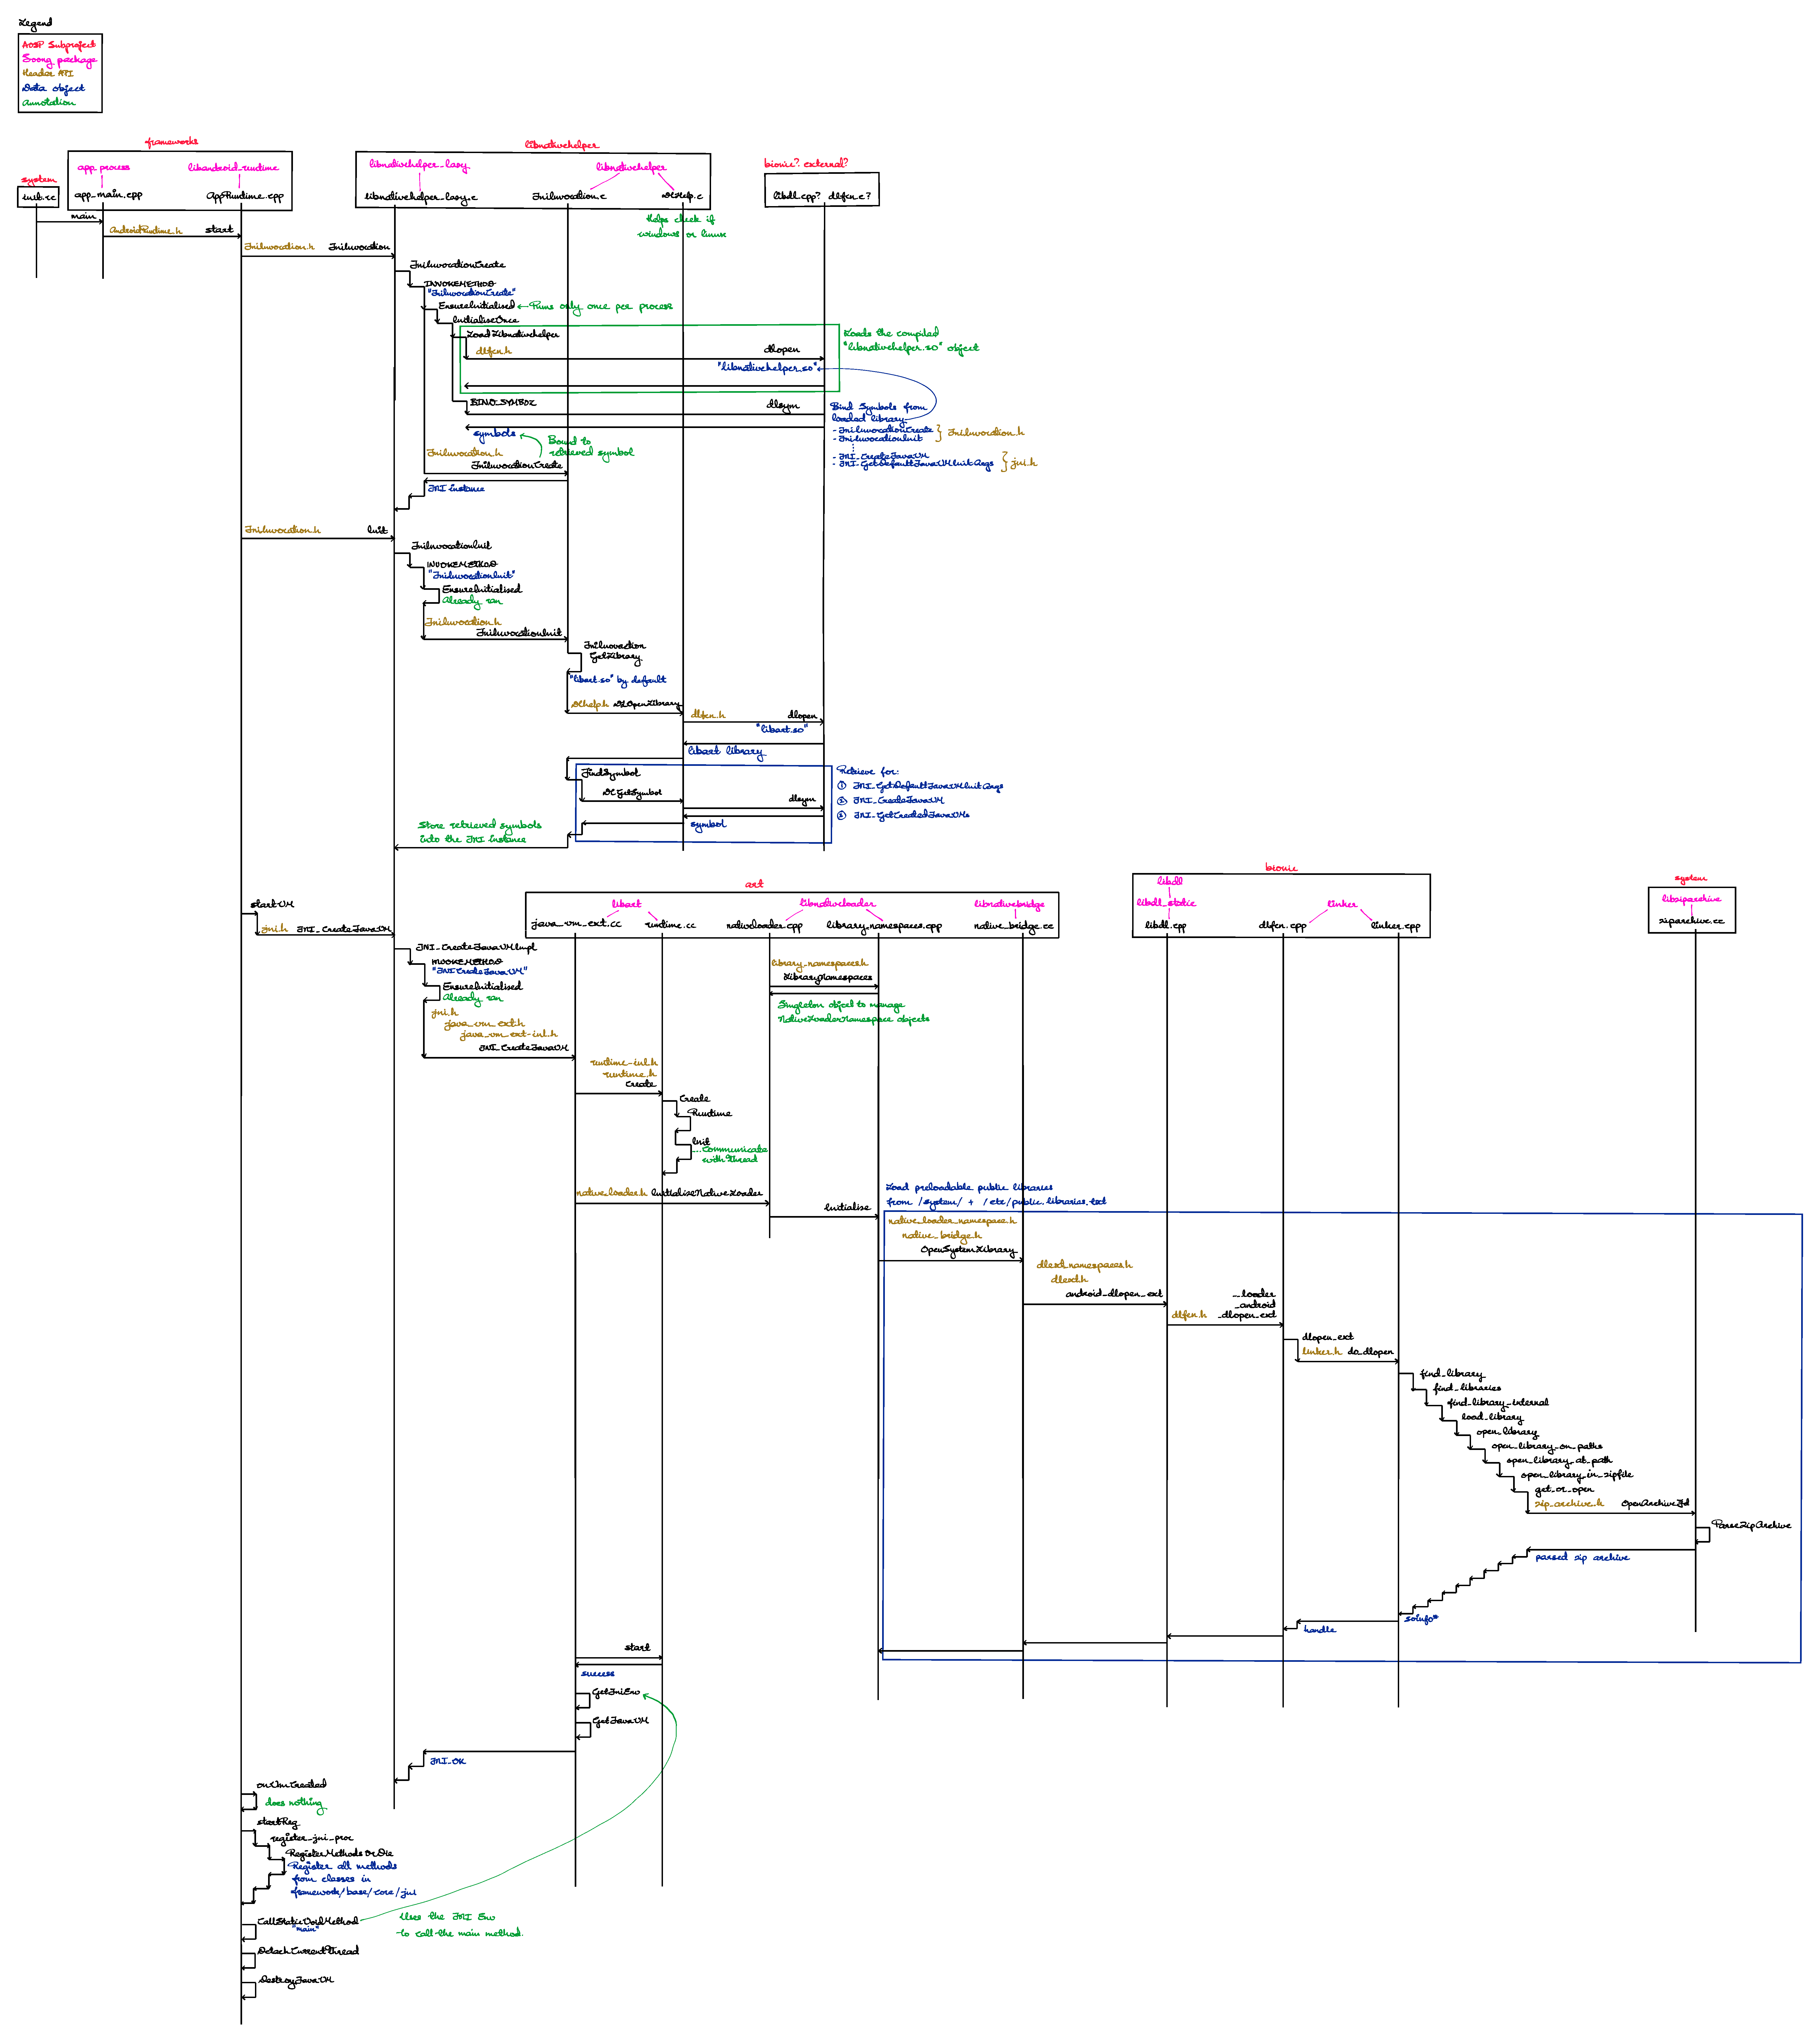
\includepdf[pages=-, scale=.95,pagecommand={}]{entries/2024/01/01/art.pdf}

% \begin{itemize}
% \item \textbf{Domain.} The context of the process that is acting upon something.
% \item \textbf{Type.} The context of the resource on which the process is acting.
% \item \textbf{Class.} The object class of the resource (e.g. \textit{file} or \textit{socket}).
% \item \textbf{Permissions.} The permissions that are allowed given the \textit{domain}, \textit{type} and \textit{class}.
% \end{itemize}

% SELinux rule syntax:


% \subsubsection{Decoding Permission Denial Message}

% Message:
% \begin{lstlisting}
% type=AVC msg=audit(1363289005.532:184): avc:  denied  { read } for  pid=29199 comm="Trace" 
% name="online" dev="sysfs" ino=30 scontext=staff_u:staff_r:googletalk_plugin_t 
% tcontext=system_u:object_r:sysfs_t tclass=file
% \end{lstlisting}

% \begin{longtable}{p{.15\linewidth}p{.15\linewidth}p{.65\linewidth}} 
% \toprule
% Log part & Name & Description \\
% \midrule
% \endhead

% \texttt{type=AVC}
% &Log type
% &Only in the \texttt{audit.log} file; it informs the user what kind of audit log type this is. 
% \\

% \texttt{msg=audit(1363289005.532:184)}
% &Timestamp
% &Timestamp in seconds since epoch, meaning the number of seconds since January 1st, 1970. You can convert this to a more human readable format using date -d @ followed by the number, like so: \texttt{date -d @1363292159.532}.
% \\

% \texttt{avc:}
% &Log type (again)
% &
% \\

% \texttt{ino=30}
% &inode number
% &The inode number of the target file. In this case, since we know it is on the \texttt{sysfs} file system, we can look for this file using: \texttt{find /sys -xdev -inum 30}
% \\

% \texttt{scontent=staff\_u:staff\_r:googletalk\_plugin\_t}
% &Source context
% &The security context of the process (the domain)
% \\

% \texttt{tcontext=system\_u:object\_r:sysfs\_t}
% &Target context
% &The security context of the target resource (in this case the file)
% \\

% \texttt{tclass=file}
% &Target class
% &The class of the target.
% \\

% \midrule
% \caption{Permission Denied Syntax} 
% \label{tab:permissiondeniedsyntax}
% \end{longtable}


% \subsubsection{SELinux Architecture}

% SELinux consists of four main components: object managers (OM), access vector cache (AVC), security server, and security policy as show below:
% \begin{figure}[H]
%     \centering
%     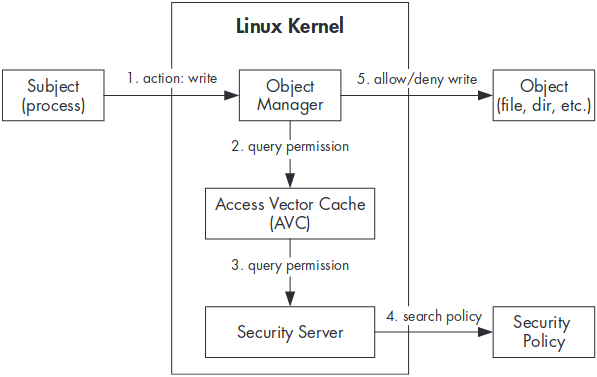
\includegraphics[width=.85\linewidth]{entries/2023/12/10/selinux.png}
%     \caption{SELinux Components}
%     \label{fig:selinux}
% \end{figure}
